% File:    report.tex
% Brief:   report for CS 354 Project 3
% Author:  G. Mcgaffin (23565608@sun.ac.za)
% Author:  J. P. Visser (21553416@sun.ac.za)
% Date:    2022-09-02


\documentclass[10pt, a4paper]{article}


\usepackage{amsmath}
\usepackage{booktabs}
\usepackage{graphicx}
\graphicspath{ {./images/exp1/}{./images/exp2/} }


\title{CS 354 Project 3: Network Address Translation}
\author{Group 41: \vspace{0.5em} \\
        G. Mcgaffin (23565608@sun.ac.za) \vspace{0.3em} \\
        J.\ P.\ Visser (21553416@sun.ac.za)}
\date{\vspace{1em} 2 September 2022}


\begin{document}


% --- Title ------------------------------------------------------------------ %

\maketitle
\newpage


% --- Table of Contents ------------------------------------------------------ %

\tableofcontents
\newpage


% --- Introduction ----------------------------------------------------------- %

\section{Introduction}
\label{sec:intro}


For this project we were tasked with implementing a simulated router with
minimal NAT functionality, as well as a simple client.

The router processes paquets received from clients, who are either marked as
internal (hosts in the local network) or external (hosts belonging to an
external network).

Clients send simple paquets to one another, and the router has to process these
paquets in an appropriate manner, depending on the following cases:
\begin{itemize}
  \item \textbf{Internal $\rightarrow$ Internal}: The paquet is forwarded
  without changing its data.
  \item \textbf{Internal $\rightarrow$ External}: The paquet header is modified
  and an entry is added to the NAT table, or refreshed if it already exists,
  that binds the source IP/port to the destination address.
  \item \textbf{External $\rightarrow$ Internal}: The paquet is routed according
  to the entry in the NAT table. If there is no corresponding entry in the table
  for the source, the paquet is dropped and an error paquet is returned (unless
  something like port forwarding has been implemented).
  \item \textbf{External $\rightarrow$ External}: Paquets are dropped, as they
  should be routed by external networks.
\end{itemize}

Additional features we needed to implement were:

\begin{itemize}
  \item \textbf{NAT table}. The address translation table should refresh
    dynamically.
  \item \textbf{DHCP}. Internal clients should automatically request and be
    assigned an address by the NAT server.
\end{itemize}


\subsection{NAT-box Requirements}
\label{ssec:natreq}

The NAT-box had the following requirements:
\begin{enumerate}
  \item The NAT-box must be given a unique hardware (MAC) address.
  \item The NAT-box must be given a unique IP address.
  \item The NAT-box’s MAC address and IP address must be communicated to
    clients.
  \item Multiple clients must be able to be connected to a single NAT-box.
  \item Internal clients must be assigned unique IP addresses by the NAT-box by
    using a minimal DHCP server implementation.
  \item If an internal client disconnects its IP address must be released into
    the pool of available IP addresses.
  \item The NAT-box must be able to process and modify the packets that it
    receives.
  \item A NAT table must be present in the implementation.
  \item The NAT table must be refreshed dynamically.
  \item The NAT table refresh time must be configurable, as this facilitates
    testing.
  \item Certain status paquets must be printed out, such as when a paquet has
    been routed, or could not be routed.
  \item Clients are only able to communicate according to the rules of the
    chosen NAT-box implementation.
\end{enumerate}


\subsection{Client Requirements}
\label{ssec:clireq}

The client implementation had the following requirements:
\begin{enumerate}
  \item Each client must either be designated as an internal or external client,
    as discussed above.
  \item A client's IP address should reflect its status as either an internal or
    external client.
  \item Internal clients should use a minimal DHCP implementation to request an
    IP address.
  \item Every client must have a unique (simulated) MAC address
  \item A client should have the ability to send a simple paquet to a targeted
    client.
  \item The client must provide a reply for every paquet received. This may take
    the form of an ACK or a similar type of packet.
  \item Clients must minimally support the following simulated protocols and
    paquets:
  \begin{enumerate}
    \item ICMP paquet forwarding (error and echo/response paquets),
    \item TU (TCP/UDP) paquet forwarding,
    \item a minimal DHCP implementation.
  \end{enumerate}
\end{enumerate}


\subsection{Overview}
\label{ssec:oview}

In this document we will provide a complete view of our implementation, by
discussing its design (\S\ref{sec:design}), giving a breakdown of the files into
which it is organized (\S\ref{sec:fdesc}), and providing a high level
description, with more details where necessary, of the flow of execution of the
two programs which it comprises (\S\ref{sec:pdesc}).

We are confident that our implementation meets all of the requirements. However,
we did not implement any features beyond those listed in the requirements
either. Therefore, we do not include sections dedicated to unimplemented or
additional features, as it would be superfluous. We also did not encounter any
serious or unexpected issues during the development process, so this topic, too,
will be excluded.

Furthermore, we will discuss experiments we have conducted (\S\ref{sec:exp}),
significant data structures (\S\ref{sec:sigds}), compilation and execution of
the router and client (\S\ref{sec:comp} and \S\ref{sec:exec}), as well as the
libraries we made use of (\S\ref{sec:libs}).


% --- File Descriptions ------------------------------------------------------ %

\section{File Descriptions}
\label{sec:fdesc}


\subsection{NAT-box/Router}
\label{ssec:natfdesc}

\begin{itemize}
  \item \texttt{NAT.java}: This file is the NAT-box's main unit. Here the
    server/router listens for new connections from clients and assigns threads
    to handle each one's incoming and outgoing traffic.
  \item \texttt{ClientHandler.java}: This file implements a handler that takes
    care of a client's input and output streams. It creates two threads, one for
    sending and the other for receiving paquets.
\end{itemize}


\subsection{Client}
\label{ssec:clifdesc}

\begin{itemize}
  \item \texttt{Client.java}: This file takes input from the user, which it uses
    to generate paquets. The paquets generated are sent to the NAT-box. It also
    receives paquets, sent by other clients, from the NAT-box and displays
    appropriate information about them to the user.
\end{itemize}


% --- Program Description ---------------------------------------------------- %

\section{Program Description}
\label{sec:pdesc}

\subsection{NAT-box/Router}
\label{ssec:natpdesc}

The following is a high-level outline of the NAT-box's flow of execution, along
with some more detailed descriptions of its operation.
\begin{enumerate}
  \item Upon startup, the NAT-box processes the command-line arguments passed to
    it. The arguments passed to it are: the port on which it must listen for new
    client connections, the maximum number of threads it is allowed to use to
    process clients, and the amount of time in milliseconds to wait before
    refreshing the NAT table.
  \item After the command-line arguments have been successfully processed, a
    listener socket is set up for clients to connect to.
  \item Once a new client has connected to the listener socket, a new thread is
    created for handling the client. The client is also added to the client
    list.
  \item A NAT table entry is created for the client's IP and port that it uses
    to listen for incoming data.
  \item The new thread then starts its execution.
  \item After handing over the client to the \texttt{ClientHandler}, the NAT-box
    then goes back to waiting for new client connections.
  \item The \texttt{ClientHandler}, once generated, creates a unique IP address
    for the client. It then sends this new IP address, the NAT's MAC address,
    and client's port number, to the client.
  \item The \texttt{ClientHandler} then waits to receive paquets sent by the
    client.
  \item Once a paquet is received, it gets processed according to the type of
    client interaction taking place:
    \begin{enumerate}
      \item \textbf{Internal $\rightarrow$ Internal}: The paquet is forwarded
        with no translation.
      \item \textbf{Internal $\rightarrow$ External}: The paquet's source
        address is translated to its assigned global address, and it is then
        forwarded to the external client.
      \item \textbf{External $\rightarrow$ Internal}: The paquet's destination
        address is translated to an internal address, and the paquet is
        forwarded to the internal client (the owner of the internal address).
      \item \textbf{External $\rightarrow$ External}: The paquet is dropped.
    \end{enumerate}
    If an address cannot be found, an ICMP paquet carrying a designated error
    message is sent to the client from which the paquet containing the unknown
    address has been received.
  \item When a client disconnects from the NAT-box, the client's socket, as well
    as input and ouput streams are closed; the client is removed from the client
    list; and its NAT table entry is discarded.
  \item When the NAT-box is terminated, each \texttt{ClientHandler} closes all
    resources used to communicate with the client that was assigned to it.
\end{enumerate}


\subsection{Client}
\label{ssec:clipdesc}

\begin{enumerate}
  \item On startup the client creates a unique MAC address for itself.
  \item It receives its assigned internal IP address, the NAT-box's MAC address,
    and the port number to use to use to communicate with the NAT-box from the
    NAT-box.
  \item Two threads are started, one for sending paquets, and another for
    receiving paquets.
  \item The receiver thread receives paquets, processes them, and displays
    relevant information to the user.
  \item The sending thread allows the user to select a type of message to send.
    The user can choose to request the client list from the NAT-box, send a ping
    to another client, or send a message to another client.
  \item Once the user has chosen an action, the appropriate paquet is generated
    and sent to the router.
  \item When the client loses connection to the NAT-box, it informs the user by
    printing a message, and terminates.
  \item On termination, all resources are closed.
\end{enumerate}


% --- Experiments ------------------------------------------------------------ %

\section{Experiments}
\label{sec:exp}


\subsection{Duplicate IP address and Port Number}
\label{ssec:dup}


\subsubsection{Experiment}
\label{sssec:dupexp}

Determine what happens when the NAT-box assigns the same IP address and port
number to two different internal clients.


\subsubsection{Hypothesis}
\label{sssec:duphyp}

Because the NAT-box uses a hash table to associate IP addresses and port numbers
with internal clients, it is expected that when an IP address and port number
that are already assigned to an internal client is assigned again to new
internal client, the new association will simply overwrite the original one. The
NAT-box and all active clients will remain operational, but there will be no way
for the original client to receive communications from any of the other clients,
since there will no longer be a NAT table entry associated with it.


\subsubsection{Test}
\label{sssec:duptest}

To test this hypothesis, introduce some small changes to the
\texttt{ClientHandler}'s source code, so that it will not generate a new IP
address and port for each new internal client, but will instead assign the same
address and port to every internal client. Then recompile and run the NAT-box.
Start three clients: two internal and one external. Then, for each client
request the client list from the NAT-box, and inspect and compare the lists.
Finally, try to send a message from the external client to the internal clients
and see what happens.


\subsubsection{Findings}
\label{sssec:dupfind}

Our hyphothesis was correct. The last internal client to connect to the NAT-box
takes over the IP address and port number from the client that connected just
before it. When sending a message to the NAT-box from the external client, only
the last connected internal client receives it. See Figures \ref{fig:exp1-1} to
\ref{fig:exp1-3}.

\begin{figure}
  \centering
  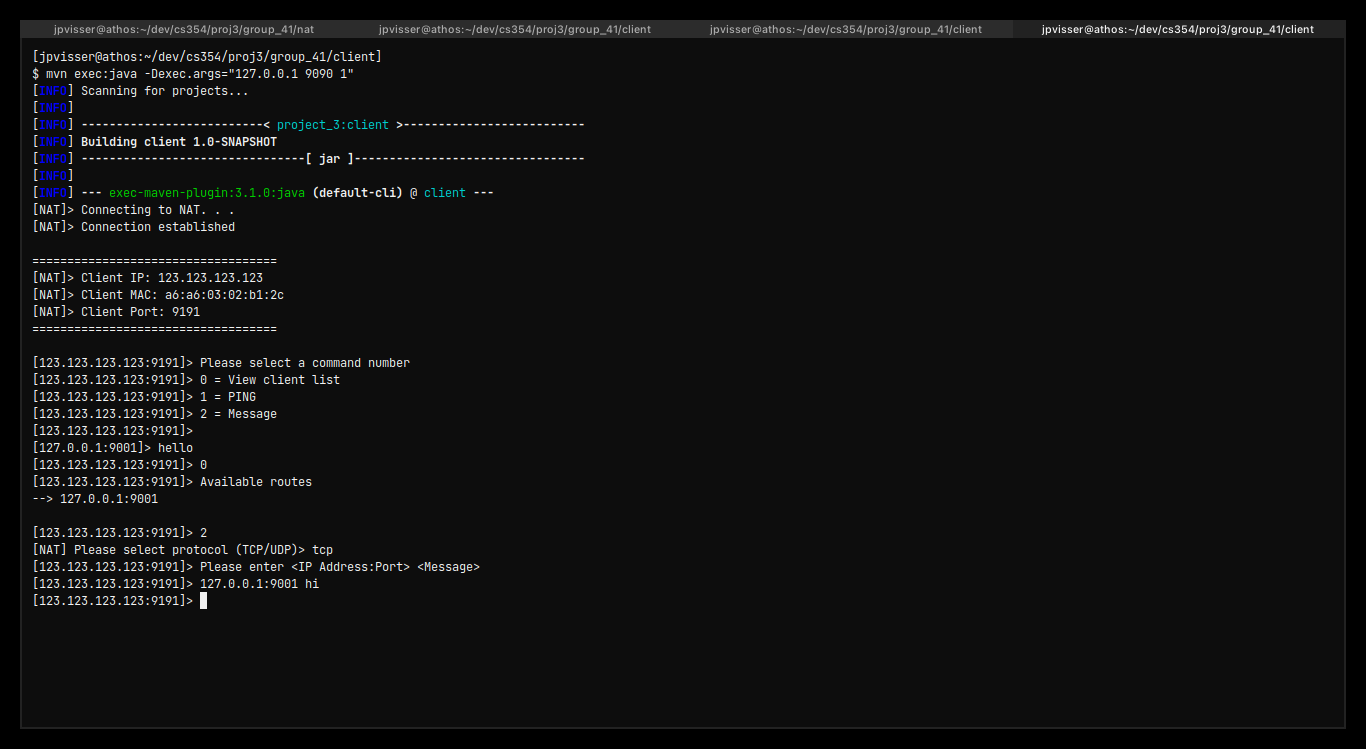
\includegraphics[width=12cm]{exp1-1}
  \caption{Message sent from the external client to the NAT-box after a
  connection between the internal and external clients has been established.}
  \label{fig:exp1-1}
\end{figure}

\begin{figure}
  \centering
  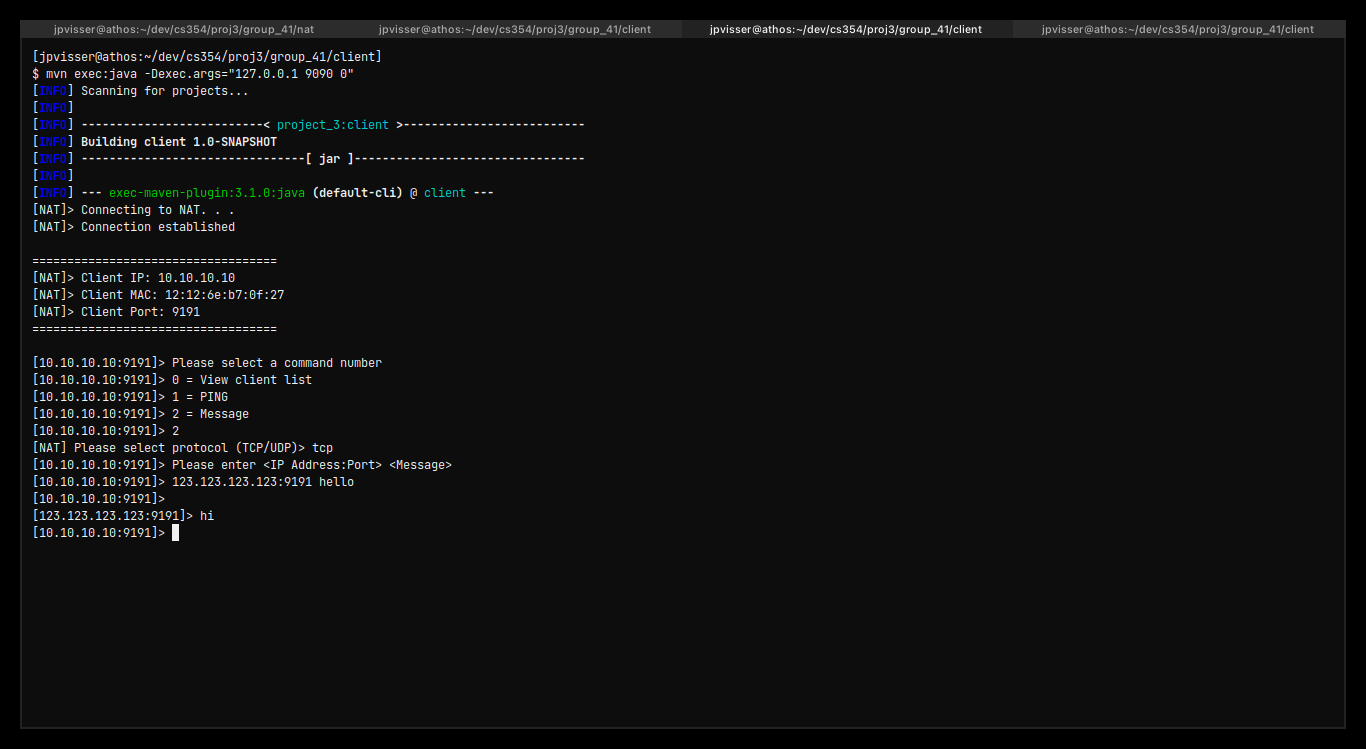
\includegraphics[width=12cm]{exp1-2}
  \caption{The last connected internal client displaying the message received
  from the external client.}
  \label{fig:exp1-2}
\end{figure}

\begin{figure}
  \centering
  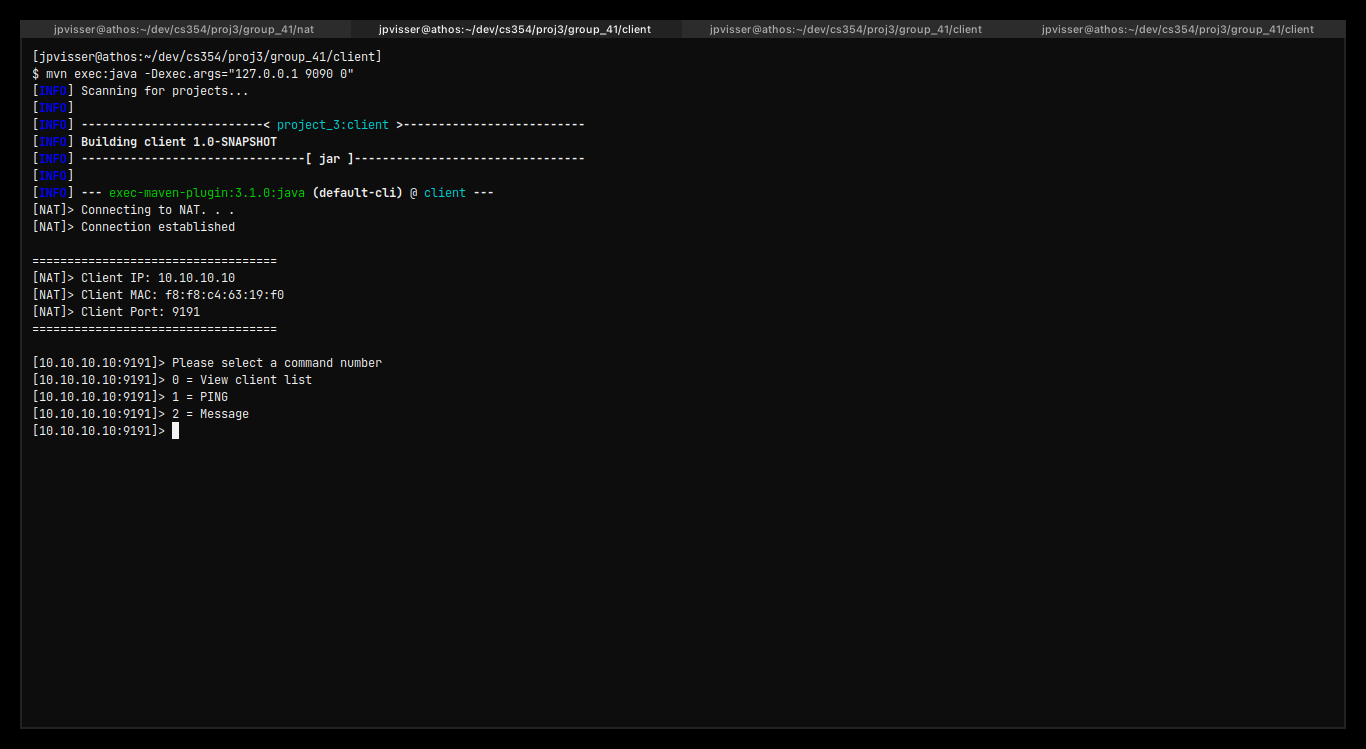
\includegraphics[width=12cm]{exp1-3}
  \caption{The client that first connected to the NAT-box shows no message,
  because the last connected client took over the IP address and port number
  from it.}
  \label{fig:exp1-3}
\end{figure}


\subsection{Too Many Clients; Too Few Threads}
\label{ssec:toomany}


\subsubsection{Experiment}
\label{sssec:toomanyexp}

Determine what happens when too many clients try to connect to the NAT-box. When
the NAT-box is run, one of its command-line arguments specifies the maximum
number of threads to use to handle clients. When the NAT-box is instructed to
use $n$ threads, but $n + 1$ clients attempt to connect, what is the result?


\subsubsection{Hypothesis}
\label{sssec:toomanyhyp}

It is expected that the last client to attempt to connect to the NAT-box will
``hang" and do nothing until one of the other clients disconnects from the
NAT-box, freeing a thread to handle the waiting client. The waiting client will
then connect to the NAT-box.


\subsubsection{Test}
\label{sssec:toomanytest}

To conduct this experiment, run the NAT-box, and specify that it must use no
more than 2 threads to handle clients. Then start up three clients. It does not
matter which types of clients are used, but we opted to use only internal
clients. One of the clients should be unable to establish a connection with the
NAT-box. Then close one of the connected clients, and observe what happens with
the aforementioned client that was unable to connect.


\subsubsection{Findings}
\label{sssec:toomanyfind}

The test disproved our hypothesis. Although the client that could not initially
connect (i.e., the third client) did ``hang" (Figure \ref{fig:exp2-1}), once one
of the other two clients disconnected, it did not successfully connect to the
NAT-box (Figure \ref{fig:exp2-3}). Also out of line with our expectations, when
the third client started up and tried to connect to the NAT-box, it caused the
NAT-box to throw a \texttt{ArrayIndexOutOfBoundsException} (Figure
\ref{fig:exp2-2}).

\begin{figure}
  \centering
  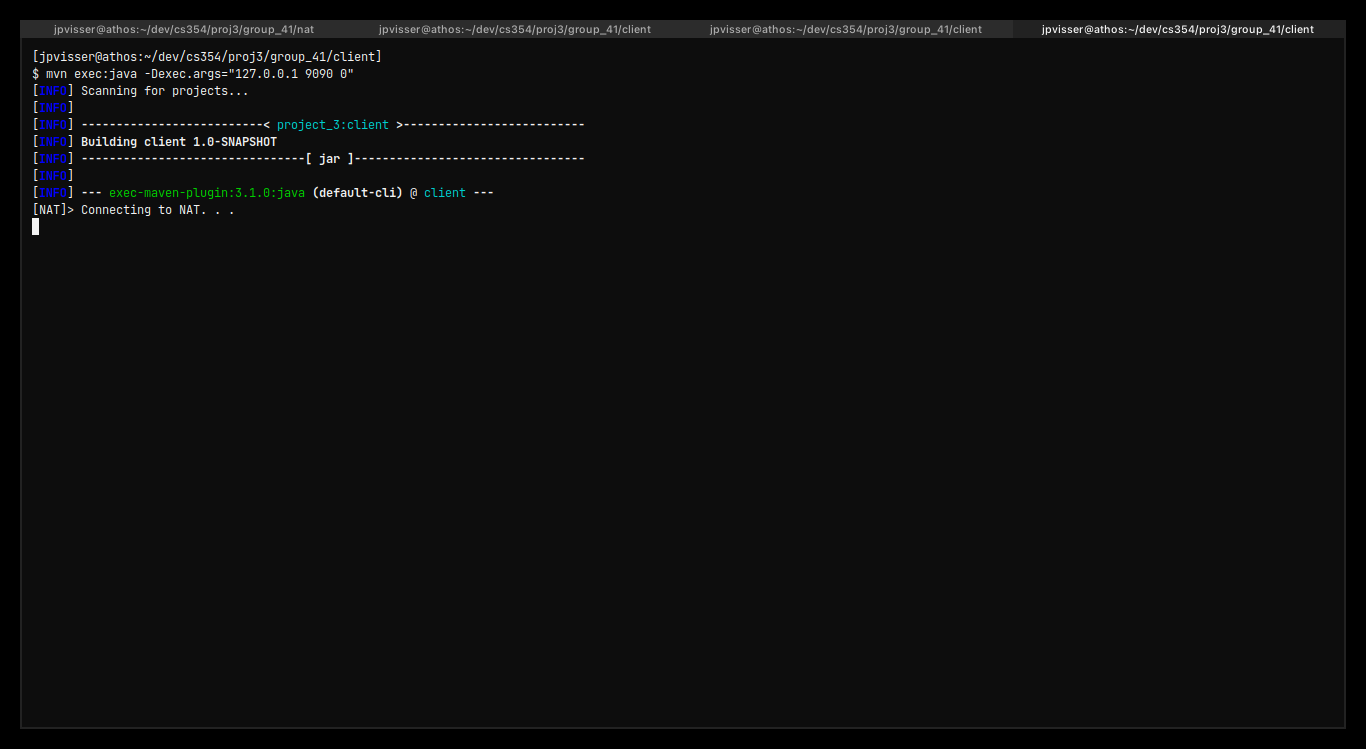
\includegraphics[width=12cm]{exp2-1}
  \caption{Third client ``hanging", unable to establish a connection with the
  NAT-box.}
  \label{fig:exp2-1}
\end{figure}

\begin{figure}
  \centering
  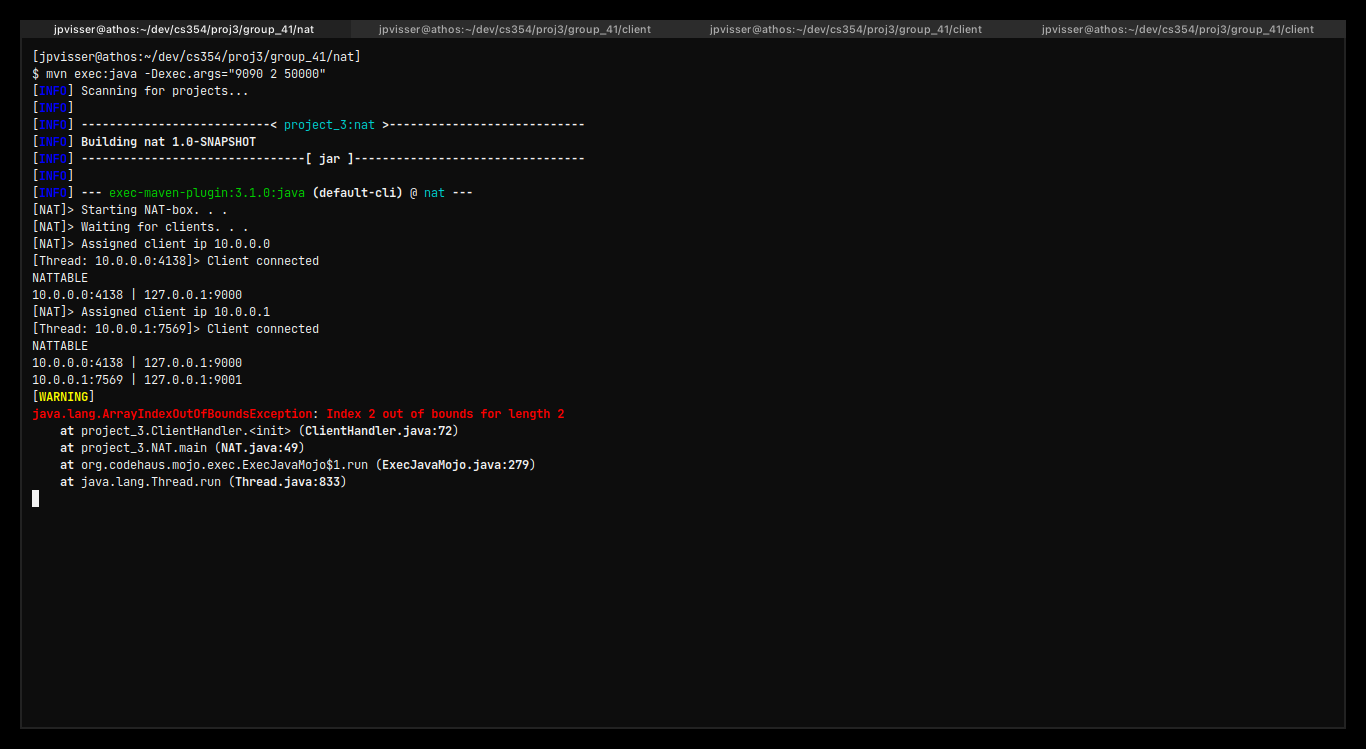
\includegraphics[width=12cm]{exp2-2}
  \caption{\texttt{ArrayIndexOutOfBoundsException} thrown by the NAT-box when
  the third client tries to connect to it.}
  \label{fig:exp2-2}
\end{figure}

\begin{figure}
  \centering
  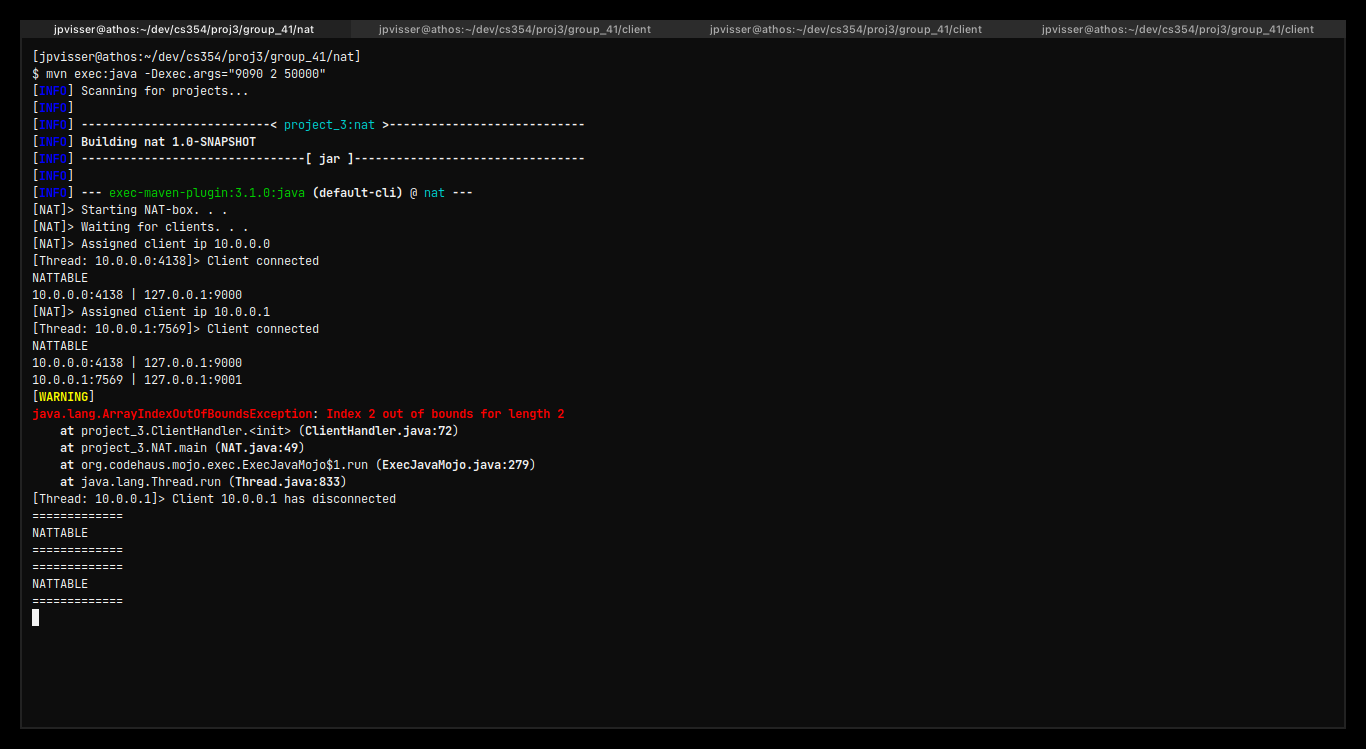
\includegraphics[width=12cm]{exp2-3}
  \caption{NAT-box output after one of the other clients disconnects.}
  \label{fig:exp2-3}
\end{figure}


% --- Significant Data Structures -------------------------------------------- %

\section{Significant Data Structures}
\label{sec:sigds}

The only data structure of note that we used for this project is the
\texttt{ConcurrentHashMap}. The \texttt{ConcurrentHashMap} is a thread safe
\texttt{HashMap} implementation. It was used to implement the NAT table and the
client list. These hash tables are accessed from multiple threads, so race
conditions can occur. The \texttt{ConcurrentHashMap} prevents this from
happening by means of synchronization.


% --- Design ----------------------------------------------------------------- %

\section{Design}
\label{sec:design}

An interesting design decision we made, was to represent paquets using byte
arrays. We took this approach, because it allows for a more realistic,
``low-level" implementation of the RFC specifications of the different types of
paquets. It resulted in an minimalistic implementation, that is efficient, and
also quick to adapt if/when necessary.


% --- Compilation ------------------------------------------------------------ %

\section{Compilation}
\label{sec:comp}

It is assumed that the project will be run on Linux from a Bash shell.


\subsection{Dependencies}
\label{ssec:deps}

In order to compile and run the NAT-box and client programs, the following
dependencies must be installed and available on the \texttt{PATH}:
\begin{itemize}
  \item OpenJDK 18.0.2
  \item Apache Maven 3.8.6
\end{itemize}
The versions listed are what we used, but older versions should work as well.


\subsection{NAT-box}
\label{ssec:compnat}

\begin{enumerate}
  \item \texttt{cd} into the \texttt{nat} directory.
  \item Compile using \texttt{mvn compile}.
\end{enumerate}


\subsection{Client}
\label{ssec:compcli}

\begin{enumerate}
  \item \texttt{cd} into the \texttt{client} directory.
  \item Compile using \texttt{mvn compile}.
\end{enumerate}


% --- Execution -------------------------------------------------------------- %

\section{Execution}
\label{sec:exec}


\subsection{NAT-box}
\label{ssec:execnat}

Run the NAT-box using the command \texttt{mvn exec:java -Dexec.args="<port> <n>
<timeout>"}, where:
\begin{itemize}
  \item \texttt{<port>} is the port number that should be used to listen for new
    client connections,
  \item \texttt{<n>} is the maximum number threads to create to handle clients,
  \item \texttt{<timeout>} is the amount of time in miliseconds to wait before
    refreshing the NAT table.
\end{itemize}


\subsection{Client}
\label{ssec:execcli}

Run the client using the command \texttt{mvn exec:java -Dexec.args="<ip> <port>
<type>"}, where:
\begin{itemize}
  \item \texttt{<ip>} is the IP address of the host that the NAT-box is running
    on;
  \item \texttt{<port>} is the port number of the NAT-box;
  \item \texttt{<type>} is the client's type, where 0 indicates an internal
    client, and 1 indicates an external client.
\end{itemize}


% --- Libraries -------------------------------------------------------------- %

\section{Libraries}
\label{sec:libs}

We used only the Java Standard API for this project.


\end{document}
